% !TeX spellcheck en_US
\documentclass{beamer}
\usepackage[utf8]{inputenc}
\usepackage[T1]{fontenc}
\usepackage{ragged2e}

\usepackage[utf8]{inputenc}  
\usepackage[T1]{fontenc}
\usepackage{geometry}
\usepackage{listings}
\usepackage{url}
\usepackage{hhline}
\usepackage[normalem]{ulem}
\usepackage[font={color=foreground,bf}]{caption}
\usepackage{array,booktabs,arydshln}
\usepackage{pdflscape}
\usepackage{xcolor}
\usepackage{inconsolata}
\usepackage{pgfplots}
\usepackage{listings}
\pgfplotsset{compat=1.17}
\usetikzlibrary{shadows}

\def\imgBaseDir{img}
\def\imgSubDir{}
\newcommand\setimgdir[1]{\def\imgSubDir{#1/}}

\newcommand\img[1]{\includegraphics[width=\linewidth]{\imgBaseDir/\imgSubDir#1}}

\newcommand\darktheme {
	
	\colorlet{foreground}{black!25}
	\colorlet{background}{black!74}
	\colorlet{focus}{yellow!50}
	\definecolor{codeColor}{RGB}{85,255,85}
	\colorlet{codeBackground}{black!80}
	\def \imgBaseDir {imgDark}
	
	
	
}
%\rowcolors{1}{background}{background!95} % Alternated array colors
%%%%%%%%%%%%%%%%%%%%%%%%%%%%%%%%%%%%%%%%%%%%%%%%%%%%%%%   BASIC STYLES   %%%%%%%%%%%%%%%%%%%%%%%%%%%%%%%%%%%%%%%%%%%%%%%%%%%%%%%
\colorlet{foreground}{black}
\colorlet{background}{white}
\colorlet{focus}{blue}
%\definecolor{codeColor}{RGB}{0,0,0}
\colorlet{codeBackground}{black!10}



\renewcommand\emph[1]	{{ \color{red!40}	\textbf{#1}} 			}
\newcommand\mynote[1]	{{ \color{focus!50} \textbf{NOTE:	} #1 }\\}
\newcommand\warning[1]	{{ \color{focus!70} \textbf{WARNING:} #1 }\\}
\newcommand\todo[1]		{{ \color{focus} 	\textbf{TODO:} 	  #1 }\\}
%%%%%%%%%%%%%%%%%%%%%%%%%%%%%%%%%%%%%%%%%%%%%%%%%%%%%%%   CODE   %%%%%%%%%%%%%%%%%%%%%%%%%%%%%%%%%%%%%%%%%%%%%%%%%%%%%%%
\lstset{
	firstnumber=1,
	texcl=true,inputencoding=latin1,
	backgroundcolor=\color{codeBackground},   % choose the background color; you must add \usepackage{color} or \usepackage{xcolor}; should come as last argument,
	basicstyle=\footnotesize\ttfamily,      % the size of the fonts that are used for the code
	breakatwhitespace=true,         % sets if automatic breaks should only happen at whitespace
	breaklines=true,
	captionpos=b,                    % sets the caption-position to bottom
	commentstyle=\color{green!65!black},    % comment style
	deletekeywords={...},            % if you want to delete keywords from the given language
	escapeinside={\%*}{*)},          % if you want to add LaTeX within your code
	extendedchars=true,              % lets you use non-ASCII characters; for 8-bits encodings only, does not work with UTF-8
	frame=single,	                   % adds a frame around the code
	keepspaces=true,                 % keeps spaces in text, useful for keeping indentation of code (possibly needs columns=flexible)
	keywordstyle=\color{blue!60},       % keyword style
	language=C,                 % the language of the code,
	morekeywords={*,...},            % if you want to add more keywords to the set
	numbers=left,                    % where to put the line-numbers; possible values are (none, left, right)
	numbersep=5pt,                   % how far the line-numbers are from the code
	numberstyle=\tiny\color{black!40}, % the style that is used for the line-numbers
	rulecolor=\color{black},         % if not set, the frame-color may be changed on line-breaks within not-black text (e.g. comments (green here))
	showspaces=false,                % show spaces everywhere adding particular underscores; it overrides 'showstringspaces'
	showstringspaces=false,          % underline spaces within strings only
	showtabs=false,                  % show tabs within strings adding particular underscores
	stepnumber=5,                    % the step between two line-numbers. If it's 1, each line will be numbered
	stringstyle=\color{violet!50},     % string literal style
	tabsize=4,	                   % sets default tabsize to 2 spaces
	title=\lstname                   % show the filename of files included with \lstinputlisting; also try caption instead of title	
}

\newcommand\icode[1]{\lstinline[breaklines=true,breakatwhitespace=false, basicstyle=\ttfamily\small]{#1}}\lstnewenvironment{code}{}{}
\lstnewenvironment{bash}{\lstset{language=Bash}}{}
\lstnewenvironment{fcode}[1]{\lstset{caption=#1}}{}

% % Environment for list in block most common case
\newenvironment{bl}[1][] % By default, no title
	{\begin{block}{#1}\begin{itemize}}
	{\end{itemize}\end{block}}


\newcolumntype{Y}{>{\centering\arraybackslash}X}


\justifying

\newcommand{\logoWidth}{1 cm}
\newcommand{\spaceh}{0,5 cm}
\colorlet{foreground}{black}
\colorlet{background}{white}
\colorlet{focus}{blue}
%\definecolor{codeColor}{RGB}{0,0,0}
\colorlet{codeBackground}{black!10}


\title{Automatic exploit generation}
\author[shortname]{
	Maxime Bélair  \inst{1} \and
	Manh-Dung Nguyen  \inst{2} \and
	Emilien Fournier \inst{3}\and
	Tristan Benoit \inst{4}\and
	Gabriel Sauger \inst{5}\\
	\vspace{0.3cm}
	\textbf{Subject by}: \large Jules Villard - 
	
\includegraphics[width = 1cm]{Figures/Logos/FacebookLogo.png}
}

\institute{
	\inst{1}%
	Orange Labs / IMT atlantique - \tiny maxime.belair@imt-atlantique.fr
	\and
	\inst{2}%
	CEA LIST \& Université Grenoble Alpes - \tiny manh-dung.nguyen@cea.fr
	\and
	\inst{3}%
	ENSTA Bretagne / Lab-STICC - \tiny emilien.fournier@ensta-bretagne.org
	\and
	\inst{4}%
	LORIA - \tiny tristan.benoit@loria.fr
	\and
	\inst{5}%
	LORIA - \tiny gabriel.sauger@loria.fr
}
\date{}

\titlegraphic{ \vspace{-1cm}
	
	
\includegraphics[width = \logoWidth]{Figures/Logos/MaxLogo1.png}
	
\includegraphics[width = 0.5cm]{Figures/Logos/MaxLogo2.png}
	\hspace{\spaceh}
	
\includegraphics[width = 0.75cm]{Figures/Logos/MDLogo1.png}
	
\includegraphics[width = \logoWidth]{Figures/Logos/MDLogo2.png}
	\hspace{\spaceh}
	
\includegraphics[width = 2.5cm]{Figures/Logos/EmilienLogo1.png}
	\hspace{0.5cm}
	
\includegraphics[width = 2CM]{Figures/Logos/GabrielLogo1.png}
	\hspace{\spaceh}
}

\usetheme{Antibes}


\setbeamertemplate{footline}[frame number]


\begin{document}
	
	\begin{frame}
	\titlepage
\end{frame}


\section{Problem overview}

% \begin{frame}
% \centering
% \LARGE

% \end{frame}

\subsection{Context}

\begin{frame}{Problem Overview}
\begin{block}{Context}
	\begin{itemize}
		\item Codebases are bigger than ever
		\item More bugs than ever!
	\end{itemize}            
\end{block}\pause

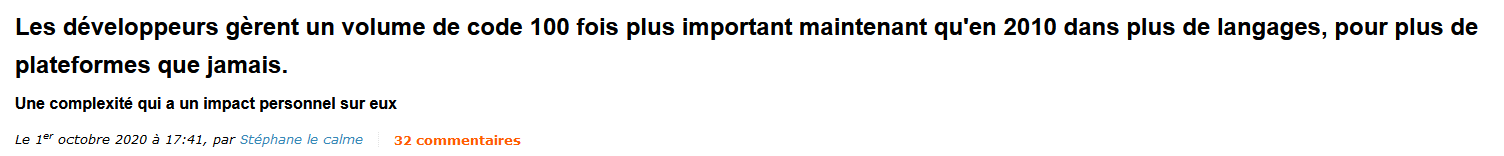
\includegraphics[width=\textwidth]{Figures/developpez.PNG} \pause

\begin{block}{Formal challenge}
	Can we automatically turn static analysis reports into executable confirming the vulnerability of a program ?
\end{block}
\end{frame}


% \begin{frame}{Context}
% \end{frame}

\subsection{Program bug example}
\begin{frame}{Program bug example}
\begin{itemize}
\item Example of vulnerability -- 101 Buffer overflow
\item Exploit it manually
\item Automatize it through infer later!
\end{itemize}
\end{frame}

\subsection{Infer tool}

\begin{frame}{Infer tool}

\begin{figure}

\includegraphics[width=\textwidth]{Figures/InferDrawing.png}
\end{figure}

\end{frame}

\begin{frame}

\begin{figure}

\includegraphics[width = 1.8cm]{Figures/InferLogo.png}

\end{figure}

\vspace{1cm}

\begin{itemize}
\item Static analysis tool from Facebook
\item \textbf{Capture} phase, then \textbf{Analysis} phase
\end{itemize}

\end{frame}

% \begin{frame}{Infer tool example}
% 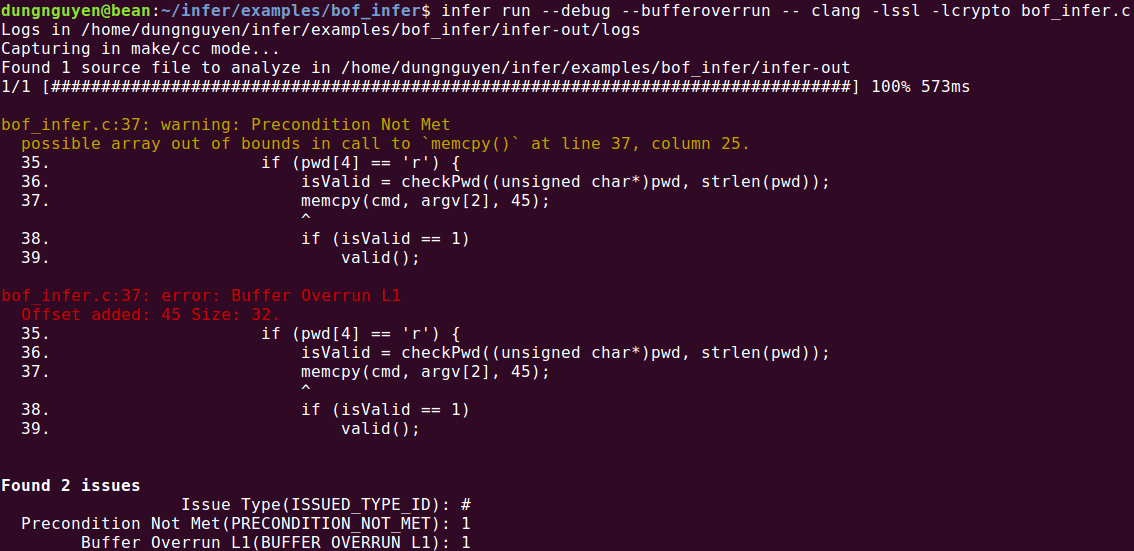
\includegraphics[width=\textwidth]{Figures/main.c/inferRunOnMain.png}
% \end{frame}

\subsection{Practical approach}



\begin{frame}{Practical approach}

\includegraphics<1>[scale=0.3]{Figures/Workflow/1.png}
\includegraphics<2>[scale=0.3]{Figures/Workflow/2.png}
\includegraphics<3>[scale=0.3]{Figures/Workflow/3.png}
\includegraphics<4>[scale=0.3]{Figures/Workflow/4.png}

\end{frame}


\begin{frame}{Practical approach}

\begin{block}{Practical challenge}
Given the Infer information about bugs of a program A, create a program B that crashes A
\end{block}

\end{frame}

\begin{frame}{Table of content}
\tableofcontents
\end{frame}

\section{Proposed approaches}

\begin{frame}
\centering

P\LARGE roposed approaches
\end{frame}


\subsection{Model checking}

\begin{frame}{Model checking }

\begin{columns}
\begin{column}{5cm}

\begin{block}{ Overview }
\begin{itemize}
\item Intuitive 
\item Automated 
\item Provides counter-examples 
\item[$\times$] State-space explosion
\end{itemize}
\end{block}

\begin{block}{}\pause
\begin{itemize}
\item Fixed-point algorithm 
\item Plenty of algorithmic variations
\end{itemize}
\end{block}

\end{column}

\begin{column}{5cm}
% \begin{block}{Overview}
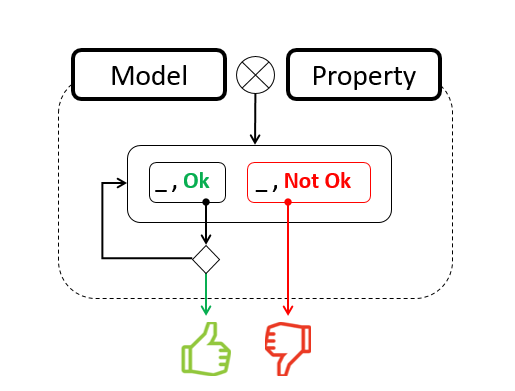
\includegraphics[width=\textwidth]{Figures/Model-checking.png}
% \end{block}
\end{column}
\end{columns}
\end{frame}


\begin{frame}
\frametitle{Application : How ? }

\includegraphics<2>[width=\textwidth]{Figures/slide_mc.png}

\begin{block}{Results}
\begin{itemize}
\item Custom model-checker
\item 16 reachability algorithms supported
\end{itemize}
\end{block}

\end{frame}





\subsection{Symbolic approach : SMT }
\begin{frame}{CFG and BFS}
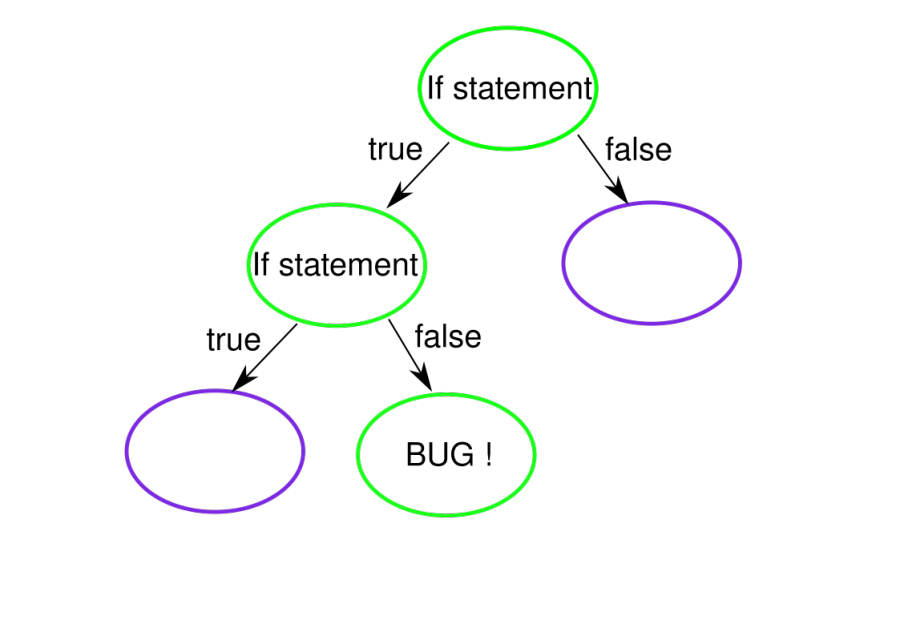
\includegraphics[width=10cm]{Figures/SMTsolver/CFG.png}

\end{frame}

\begin{frame}{Compiler}
\textbf{SmallFoot} to \textbf{SMT-LIB2}
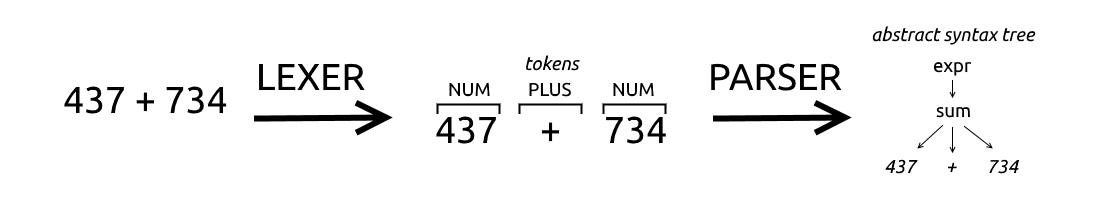
\includegraphics[width=10cm]{Figures/SMTsolver/Image_PARSER_LEXER.png}

\end{frame}

\begin{frame}{SMT solver}
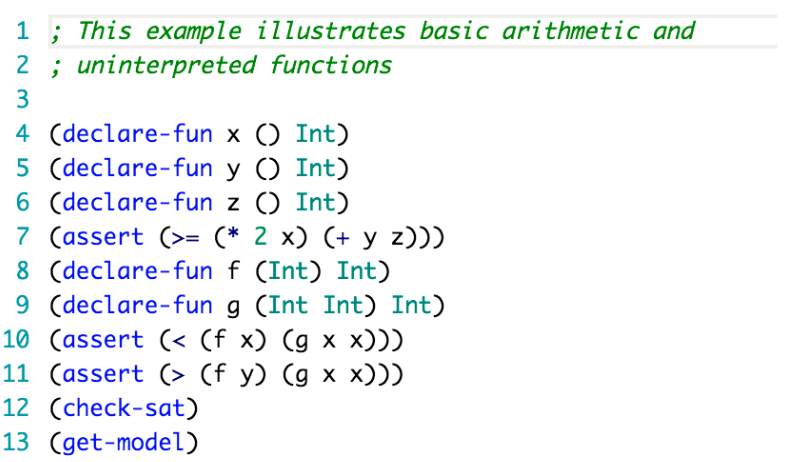
\includegraphics[width=10cm]{Figures/SMTsolver/SAT_SMTLIB.png}
\end{frame}

\begin{frame}{Flowchart}
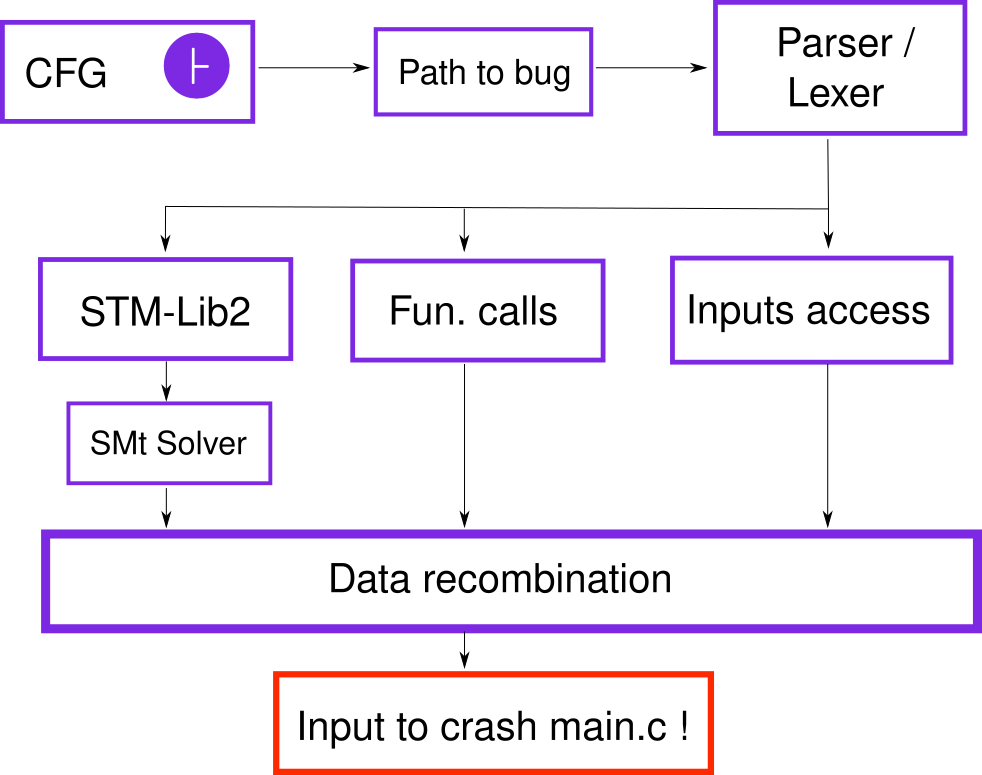
\includegraphics[width=10cm]{Figures/SMTsolver/SMTsolverCompete.png}
\end{frame}

\begin{frame}{Data recombination}

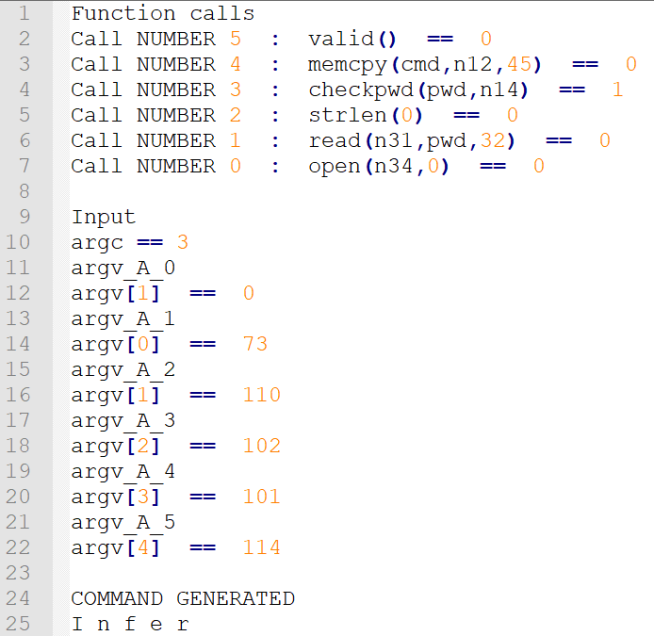
\includegraphics[width=10cm]{Figures/SMTsolver/Reports.png}

\end{frame}

\subsection{Fuzzing technique}

\begin{frame}{Fuzzing technique}

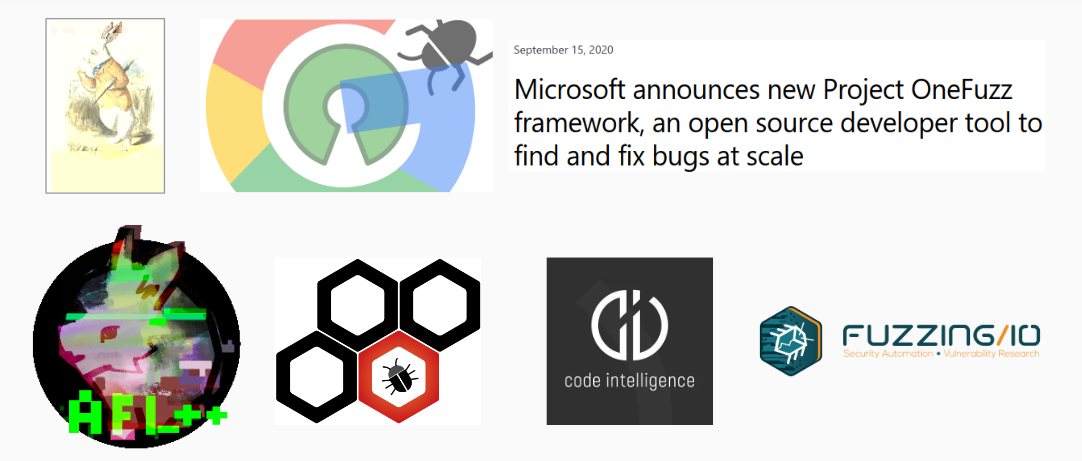
\includegraphics[width=11.5cm]{Figures/Fuzzing/graph1.png}
\centering\textbf{> 100 fuzzers} in recent years
\end{frame}

\begin{frame}{Coverage-guided greybox fuzzing}
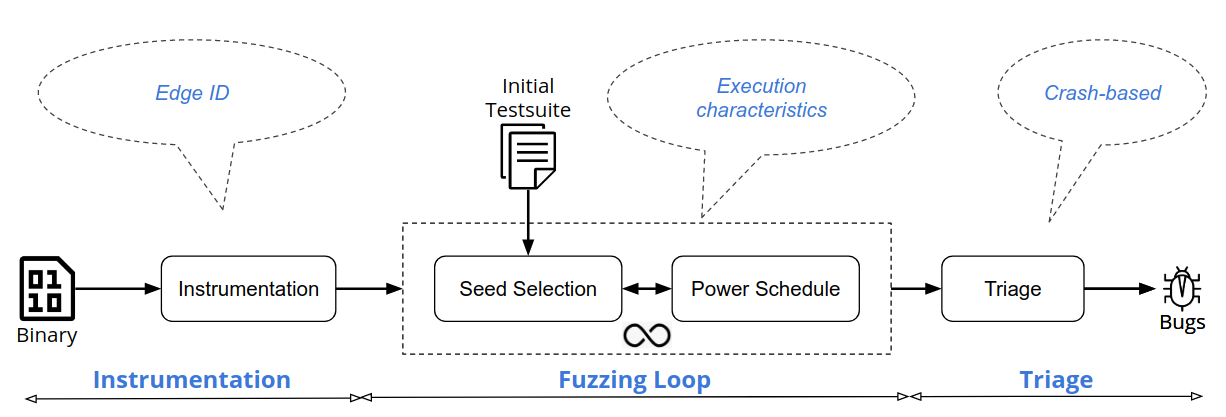
\includegraphics[width=11.5cm]{Figures/Fuzzing/graph2.png}

\centering Goal: Cover as many paths as possible\\
\centering Leverage code coverage (e.g., lines, branches) to guide the fuzzer
\end{frame}

\begin{frame}{Intuitions of Directed greybox fuzzing}
\begin{itemize}
\item Goal: Reach predefined targets (e.g., recent code changes, vulnerable functions, patches)
\item New distance-based input metric
\item Favor inputs that are "closer" to targets (select more often, produce more mutants from those inputs)
\end{itemize}
\end{frame}

\begin{frame}{Directed greybox fuzzing}
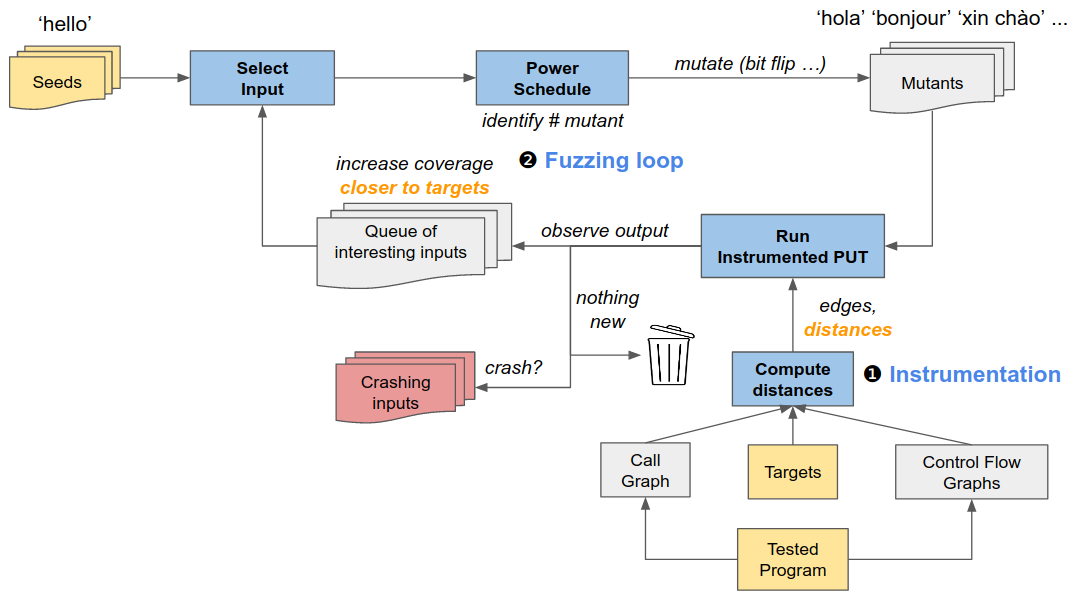
\includegraphics[width=11.5cm,height=7cm]{Figures/Fuzzing/graph3.png}

\end{frame}

\begin{frame}{Fuzzing technique}

\includegraphics<1>[scale=0.3]{Figures/Fuzzing/1.png}
\includegraphics<2>[scale=0.3]{Figures/Fuzzing/2.png}
\includegraphics<3>[scale=0.3]{Figures/Fuzzing/3.png}
\includegraphics<4>[scale=0.3]{Figures/Fuzzing/4.png}
\includegraphics<5>[scale=0.3]{Figures/Fuzzing/5.png}

\end{frame}

\begin{frame}{Result}
\begin{itemize}
\item Implementation: a Python script to parse Infer's output \& generate a script to automatically run AFLGo
\item Evaluation: run 5 times due to randomness
\end{itemize}

\end{frame}


\section{Conclusions and perspectives}

\begin{frame}
\centering
\LARGE Conclusions and perspectives
\end{frame}

\subsection{Results comparison}

\begin{frame}{Results comparison}

\textit{Show a table approaches / program comparing results (yes/no, running time, implementation complexity, computational complexity } \\

\end{frame}

\subsection{Future Work}
\begin{frame}{Future work}

Put eeeeeverything we think of. Ex:

\begin{itemize}
\item Create a fully automatic process
\item \textbf{SMT approach}: Manage fonctions calls in main.c 
\end{itemize}

\end{frame}

\begin{frame}{Future Work}
\textit{Add a graph of automatic exploits using expert models}
\end{frame}

\begin{frame}
\frametitle{Future Work -- Automatic exploit generation}
\begin{itemize}
\item We go to bugs
\item How to exploit them?
\item Create an expert code
\item Translate it to graph
\item Find all possible exploits with the same graph algorithms
\item $\to$ FULLY AUTOMATED EXPLOITS!
\end{itemize}
\end{frame}

\begin{frame}[fragile]
\frametitle{Convert vulnerabilities to bug}
\begin{code}
void onBufferOverflow(struct infer_env* env, unsigned int bufsz, unsigned long entrypoint) {
if(bufSz > (off($rip) - &entry))
addExploit("Can rewrite on $rip");
for(int var=0;  var < env.payload_nb_vars; ++var)
if( env.payload_vars.rewrittable && env.payload_vars.used)
addExploit("Can Hijack the program");
/* [...]  */
}
\end{code}
\end{frame}

\begin{frame}
\frametitle{Future Work -- Automatic exploit generation}
\tikzstyle{arrow} = [thick,->,>=stealth]
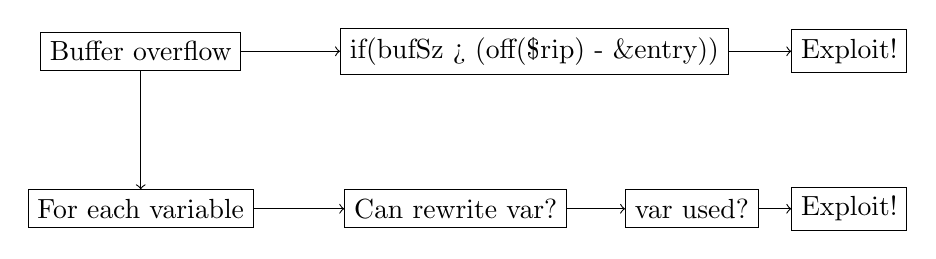
\begin{tikzpicture}
\node at (0,0) [rectangle,draw] (s) {Buffer overflow};
\node at (5,0) [rectangle,draw] (a1) {if(bufSz > (off(\$rip) - \&entry))};
\node at (9,0) [rectangle,draw] (a2) {Exploit!};
\node at (0,-2) [rectangle,draw] (b1) {For each variable};
\node at (4,-2) [rectangle,draw] (b2) {Can rewrite var?};
\node at (7,-2) [rectangle,draw] (b3) {var used?};
\node at (9,-2) [rectangle,draw] (b4) {Exploit!};
\draw[->] (s) -- (a1);
\draw[->] (a1) -- (a2);
\draw[->] (s) -- (b1) ;
\draw[->] (b1) -- (b2);
\draw[->] (b2)-- (b3) ;
\draw[->](b3) -- (b4);
\end{tikzpicture}

\end{frame}

\begin{frame}
\frametitle{Other Approaches -- Hybrid methods}
\begin{itemize}
\item Hybrid methods
\begin{itemize}
\item Prune interesting branches with Fuzzing + Heuristics
\item SMT on subproblems
\item Allow to work on bigger projects
\end{itemize}
\end{itemize}
\end{frame}

\begin{frame}{Recap}

\begin{columns}
	\column{0.333\textwidth}
	SMT
	\begin{itemize}
		\item[+] Rapide
		\item[+] Complexité des fonctions 
		\item[--] Limitations sémantiques
	\end{itemize}
	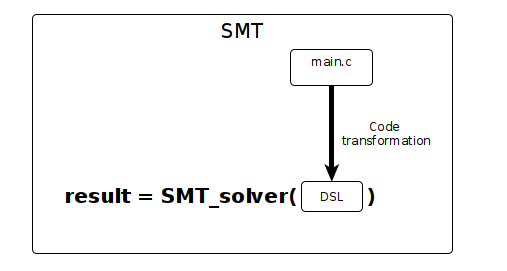
\includegraphics[width=\textwidth]{Figures/SMT_sumup}
	
	\column{0.333\textwidth} 
	Fuzzing
	\begin{itemize}
		\item[+] Can be efficent
		\item[--] Does not always find the solution
	\end{itemize}
	
	\includegraphics[width=\textwidth]{Figures/Fuzzing_sumup}    
	\column{0.333\textwidth}
	Model Checking
	\begin{itemize}
		\item[+] Sémantique 
		\item[--] Explosion combinatoire
		
	\end{itemize}
	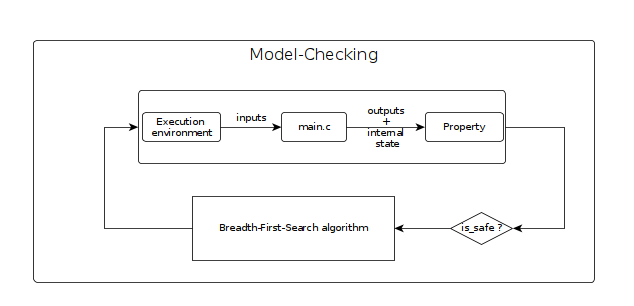
\includegraphics[width=\textwidth]{Figures/sumup_MC}
\end{columns}


\end{frame}

\begin{frame}
\frametitle{Improve the framework}
\begin{itemize}
\item Fuzzing
\begin{itemize}
\item Resolve magic-bytes comparisions, e.g., \icode{strcmp}
\item Distance computation is long with large programs
\end{itemize}
\item SMT
\begin{itemize}
\item Add more types
\item Support arbitrary memory accesses
\item Improve function with hooks	
\end{itemize}
\item Solver
\begin{itemize}
\item CCCC
\end{itemize}
\end{itemize}
\end{frame}
\begin{frame}{It works on my machine}
\begin{center}

\includegraphics[height=\textheight]{Figures/Compilation}
\end{center}


\end{frame}

\begin{frame}{Thank you !}


\includegraphics[width=\textwidth]{Figures/Questions}

\end{frame}



\end{document}
